\chapter{Integration Tests} 
\label{chap:integration_tests}

The following chapter will focus on the main sequence of events that the
autoscaler goes through to scale its consumer group. 

\begin{figure}[H]
\centering
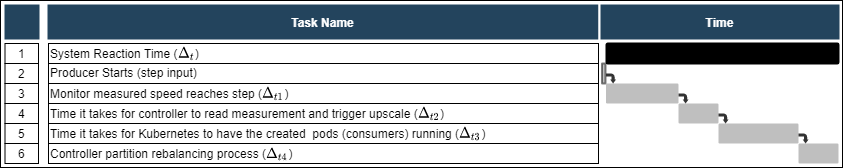
\includegraphics[width=\textwidth]{images/integration/integration_gant.png}
\caption{System sequence of events.}
\label{fig:step_event_sequence}
\end{figure}

The time it takes the controller to react to a certain measurement depends on
all the events presented in figure \ref{fig:step_event_sequence}. The following
sections will delve into each of these events. 

The data points presented for each $\Delta_{tn}, \ n \in \{1, 2, 3, 4\}$, were
obtained by testing the system with various simulations of step inputs, and
randomly generated sequences of measurements similar to the sequences used in
section \ref{c3subsub:testing}.

\section{Monitor Measurement Convergence Time}
\label{c3sec:MonitorMeasurement}

To evaluate the monitor's response time, the data points were obtained by
feeding the system a step input, which is obtained by starting a producer that
sends data to one of the partitions the consumer group is consuming data from.

\begin{figure}[H]
\centering
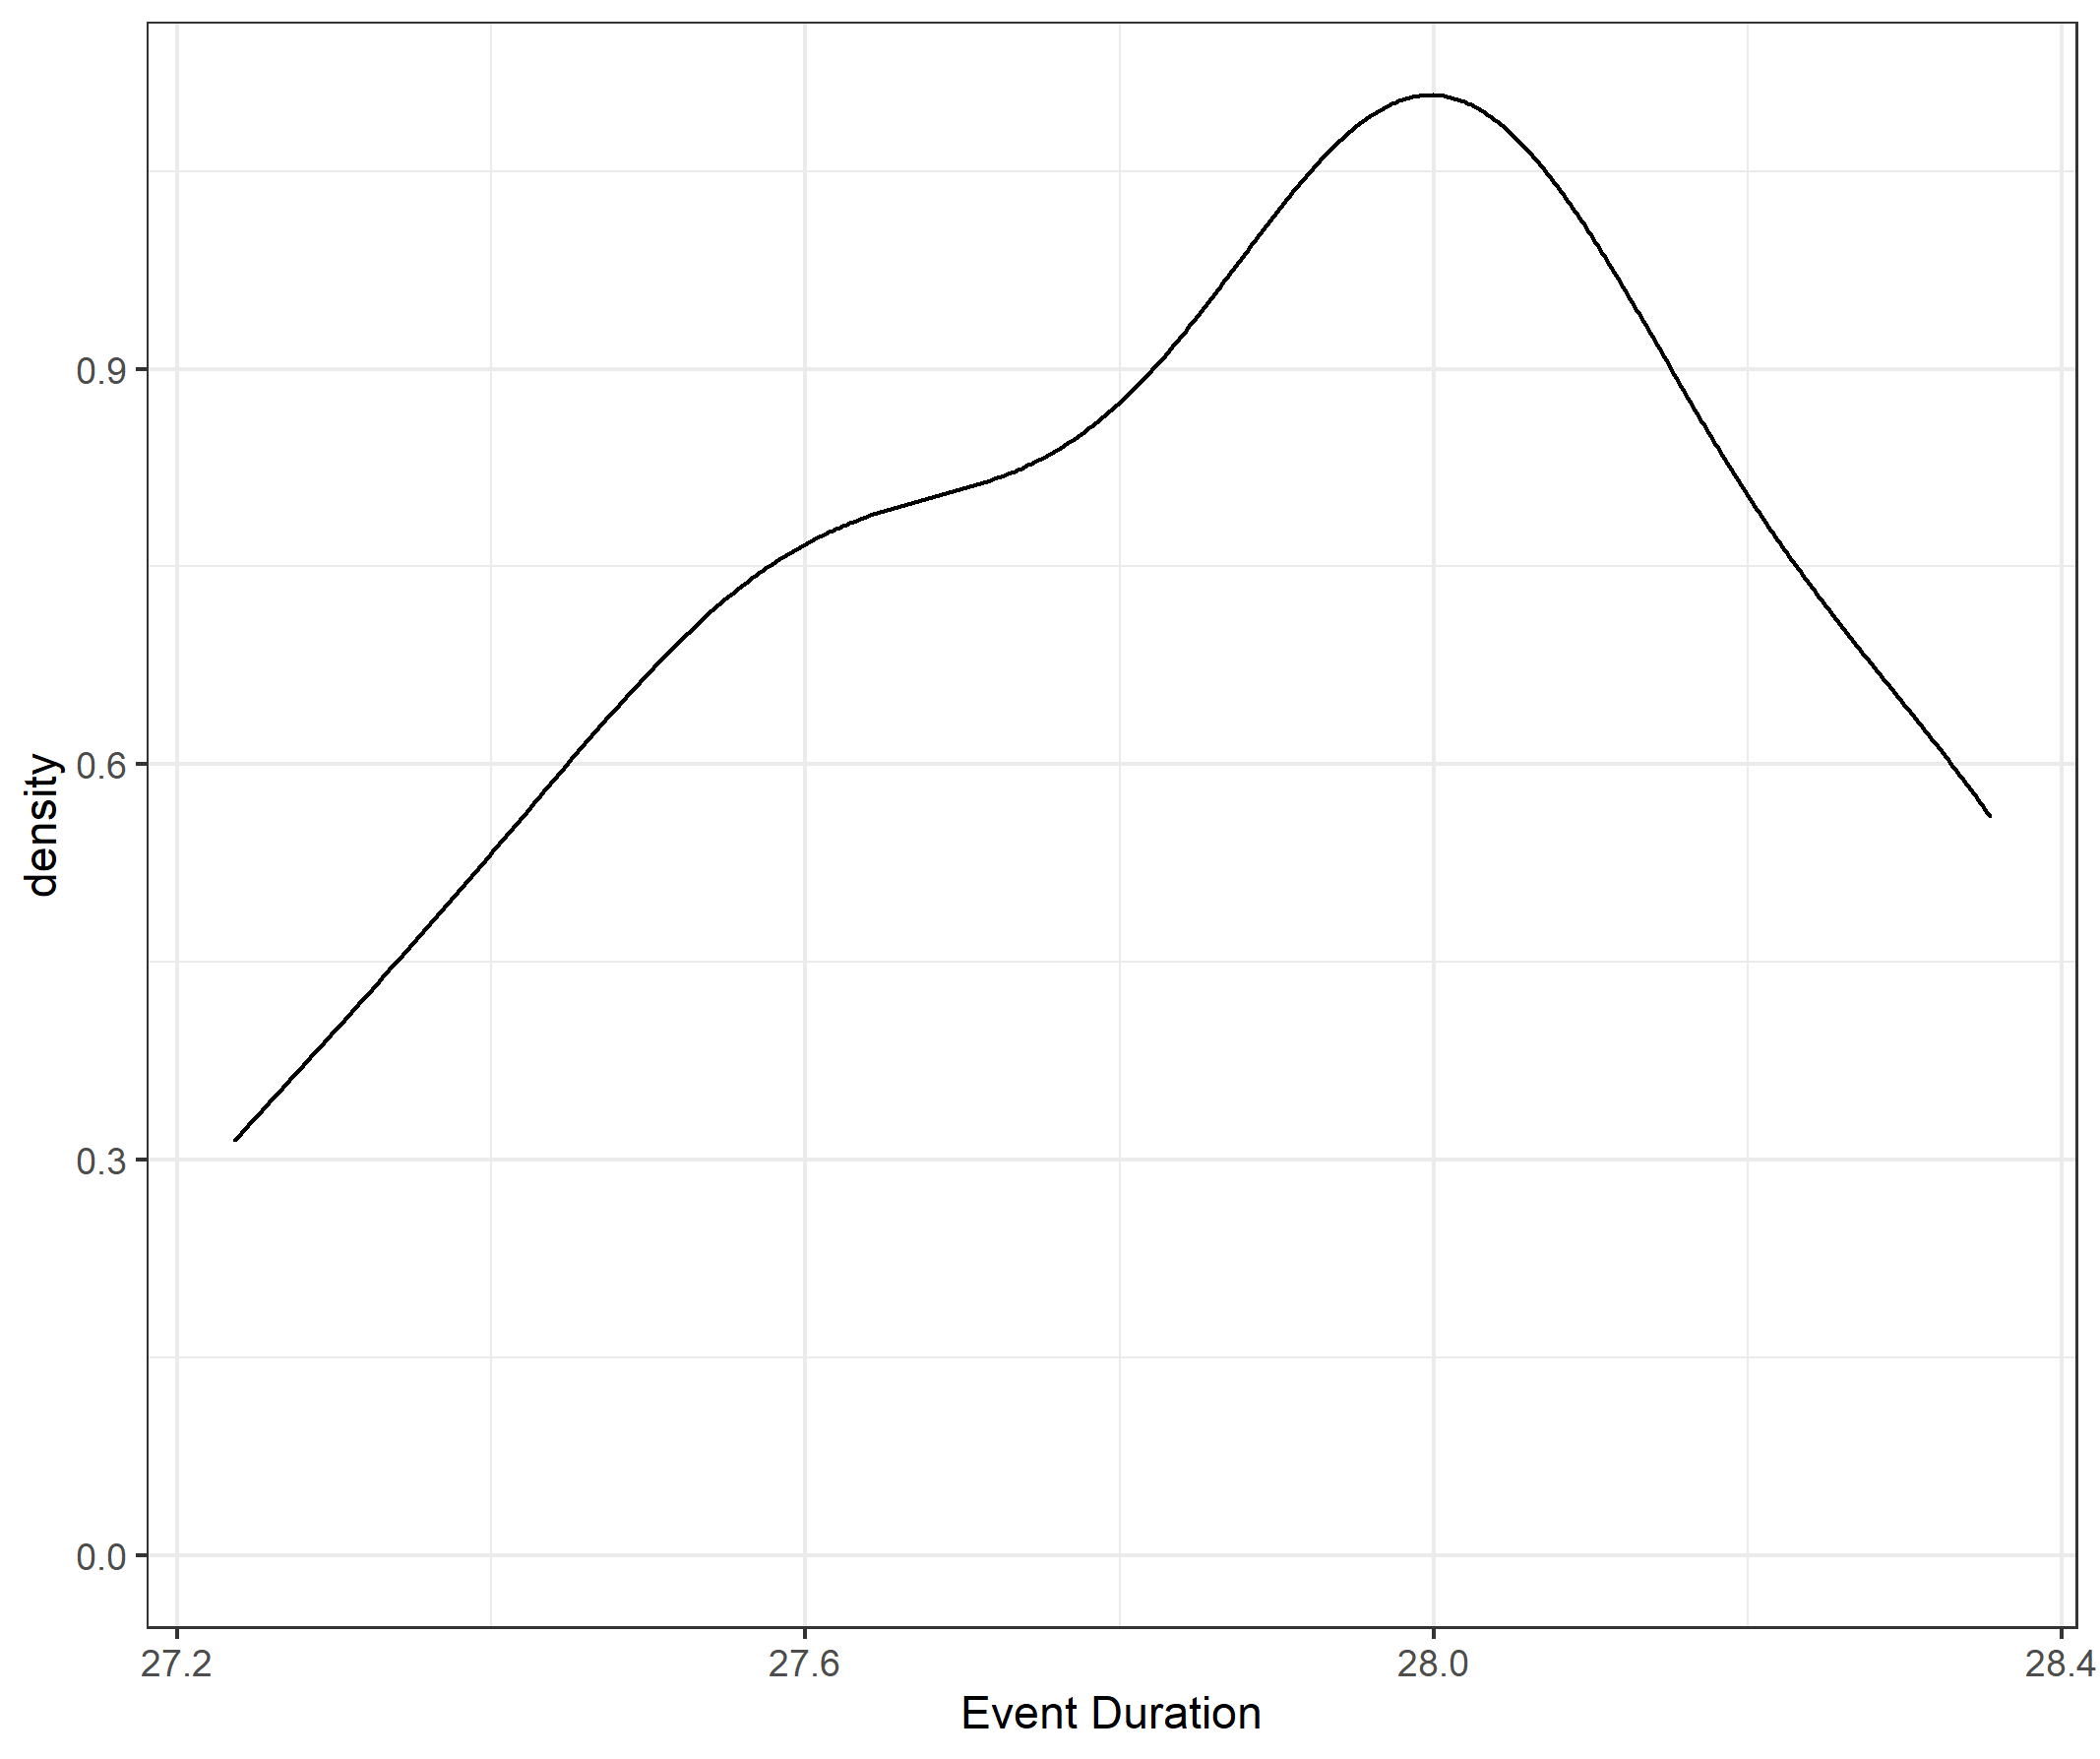
\includegraphics[width=0.6\textwidth]{images/integration/delta1.png}
\caption{Distribution of the time it takes the monitor process to reach the step value for 33 different step inputs.}
\label{fig:controller_result_monitor}
\end{figure}

As such, this measure is the time it takes the monitor process to converge to
the real production rate, which, as can be verified in figure
\ref{fig:controller_result_monitor}, takes no more than $30s$, similar to what
had been obtained in figure \ref{fig:monitor_step}.

\section{Time to Trigger Scale-up}

Measured as the time it takes the controller to compute the consumer group's new
assignment, and to send an asynchronous request to the GKE cluster for every new
consumer instance to be created. To obtain the distribution for this metric, the
system was tested with the aforementioned step inputs and the randomly generated
measurement sequences.

\begin{figure}[htb!]
\centering
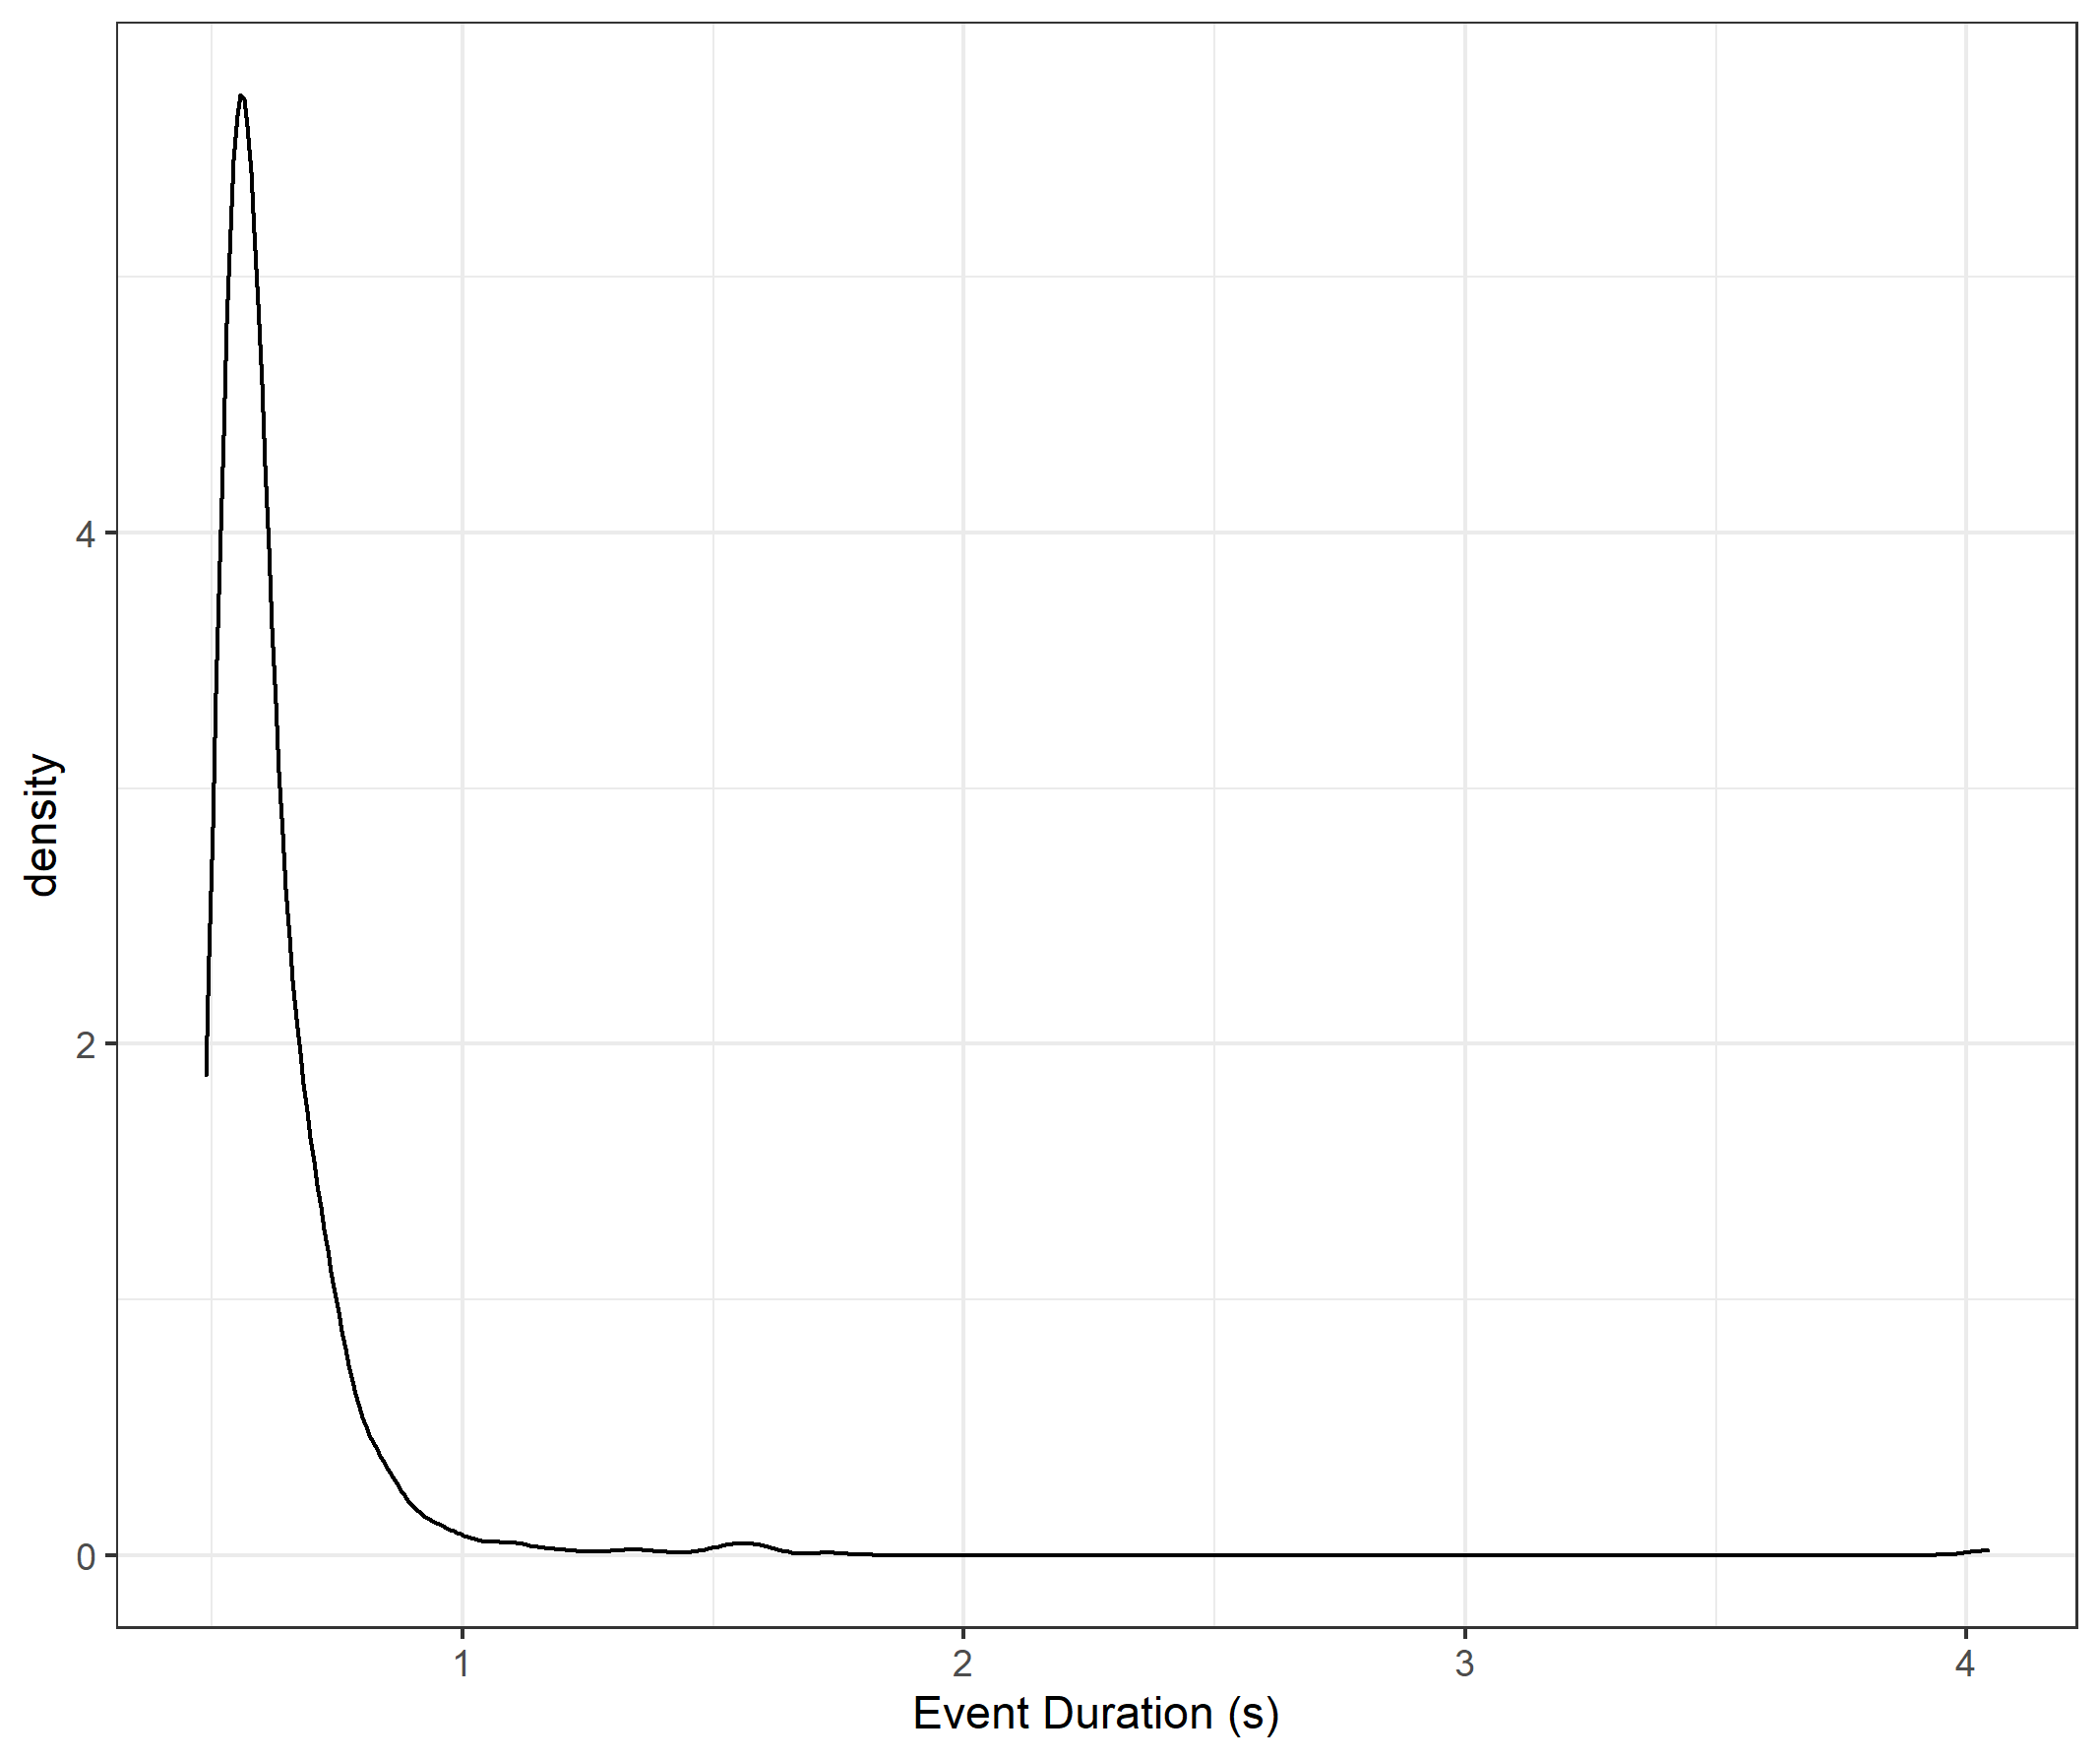
\includegraphics[width=0.6\textwidth]{images/integration/delta2.png}
\caption{
    Distribution of the time it takes the controller to compute a new
    consumer group state and send the asynchronous request to create the new
    consumers to the kubernetes cluster.
}
\label{fig:controller_result_trigger}
\end{figure}

The time the controller takes with this procedure depends on the number of
partitions to distribute between the consumer group, the algorithm the
controller is executing to figure a new consumer group assignment, and the
number of new consumer instances it has to create in the GKE cluster.

For the tested input data, where there were at most 32 partitions to rebalance
and no more than 20 consumers to be created in a single instance, the event
consistently takes less than 1 second to be executed as shown in figure
\ref{fig:controller_result_trigger}.

\section{Newly Created Deployments Ready}

After making the asynchronous request to the GKE cluster, the control plane
schedules the pods to a node, and within the node starts the containers that are
to be executed.

\begin{figure}[htb!]
\centering
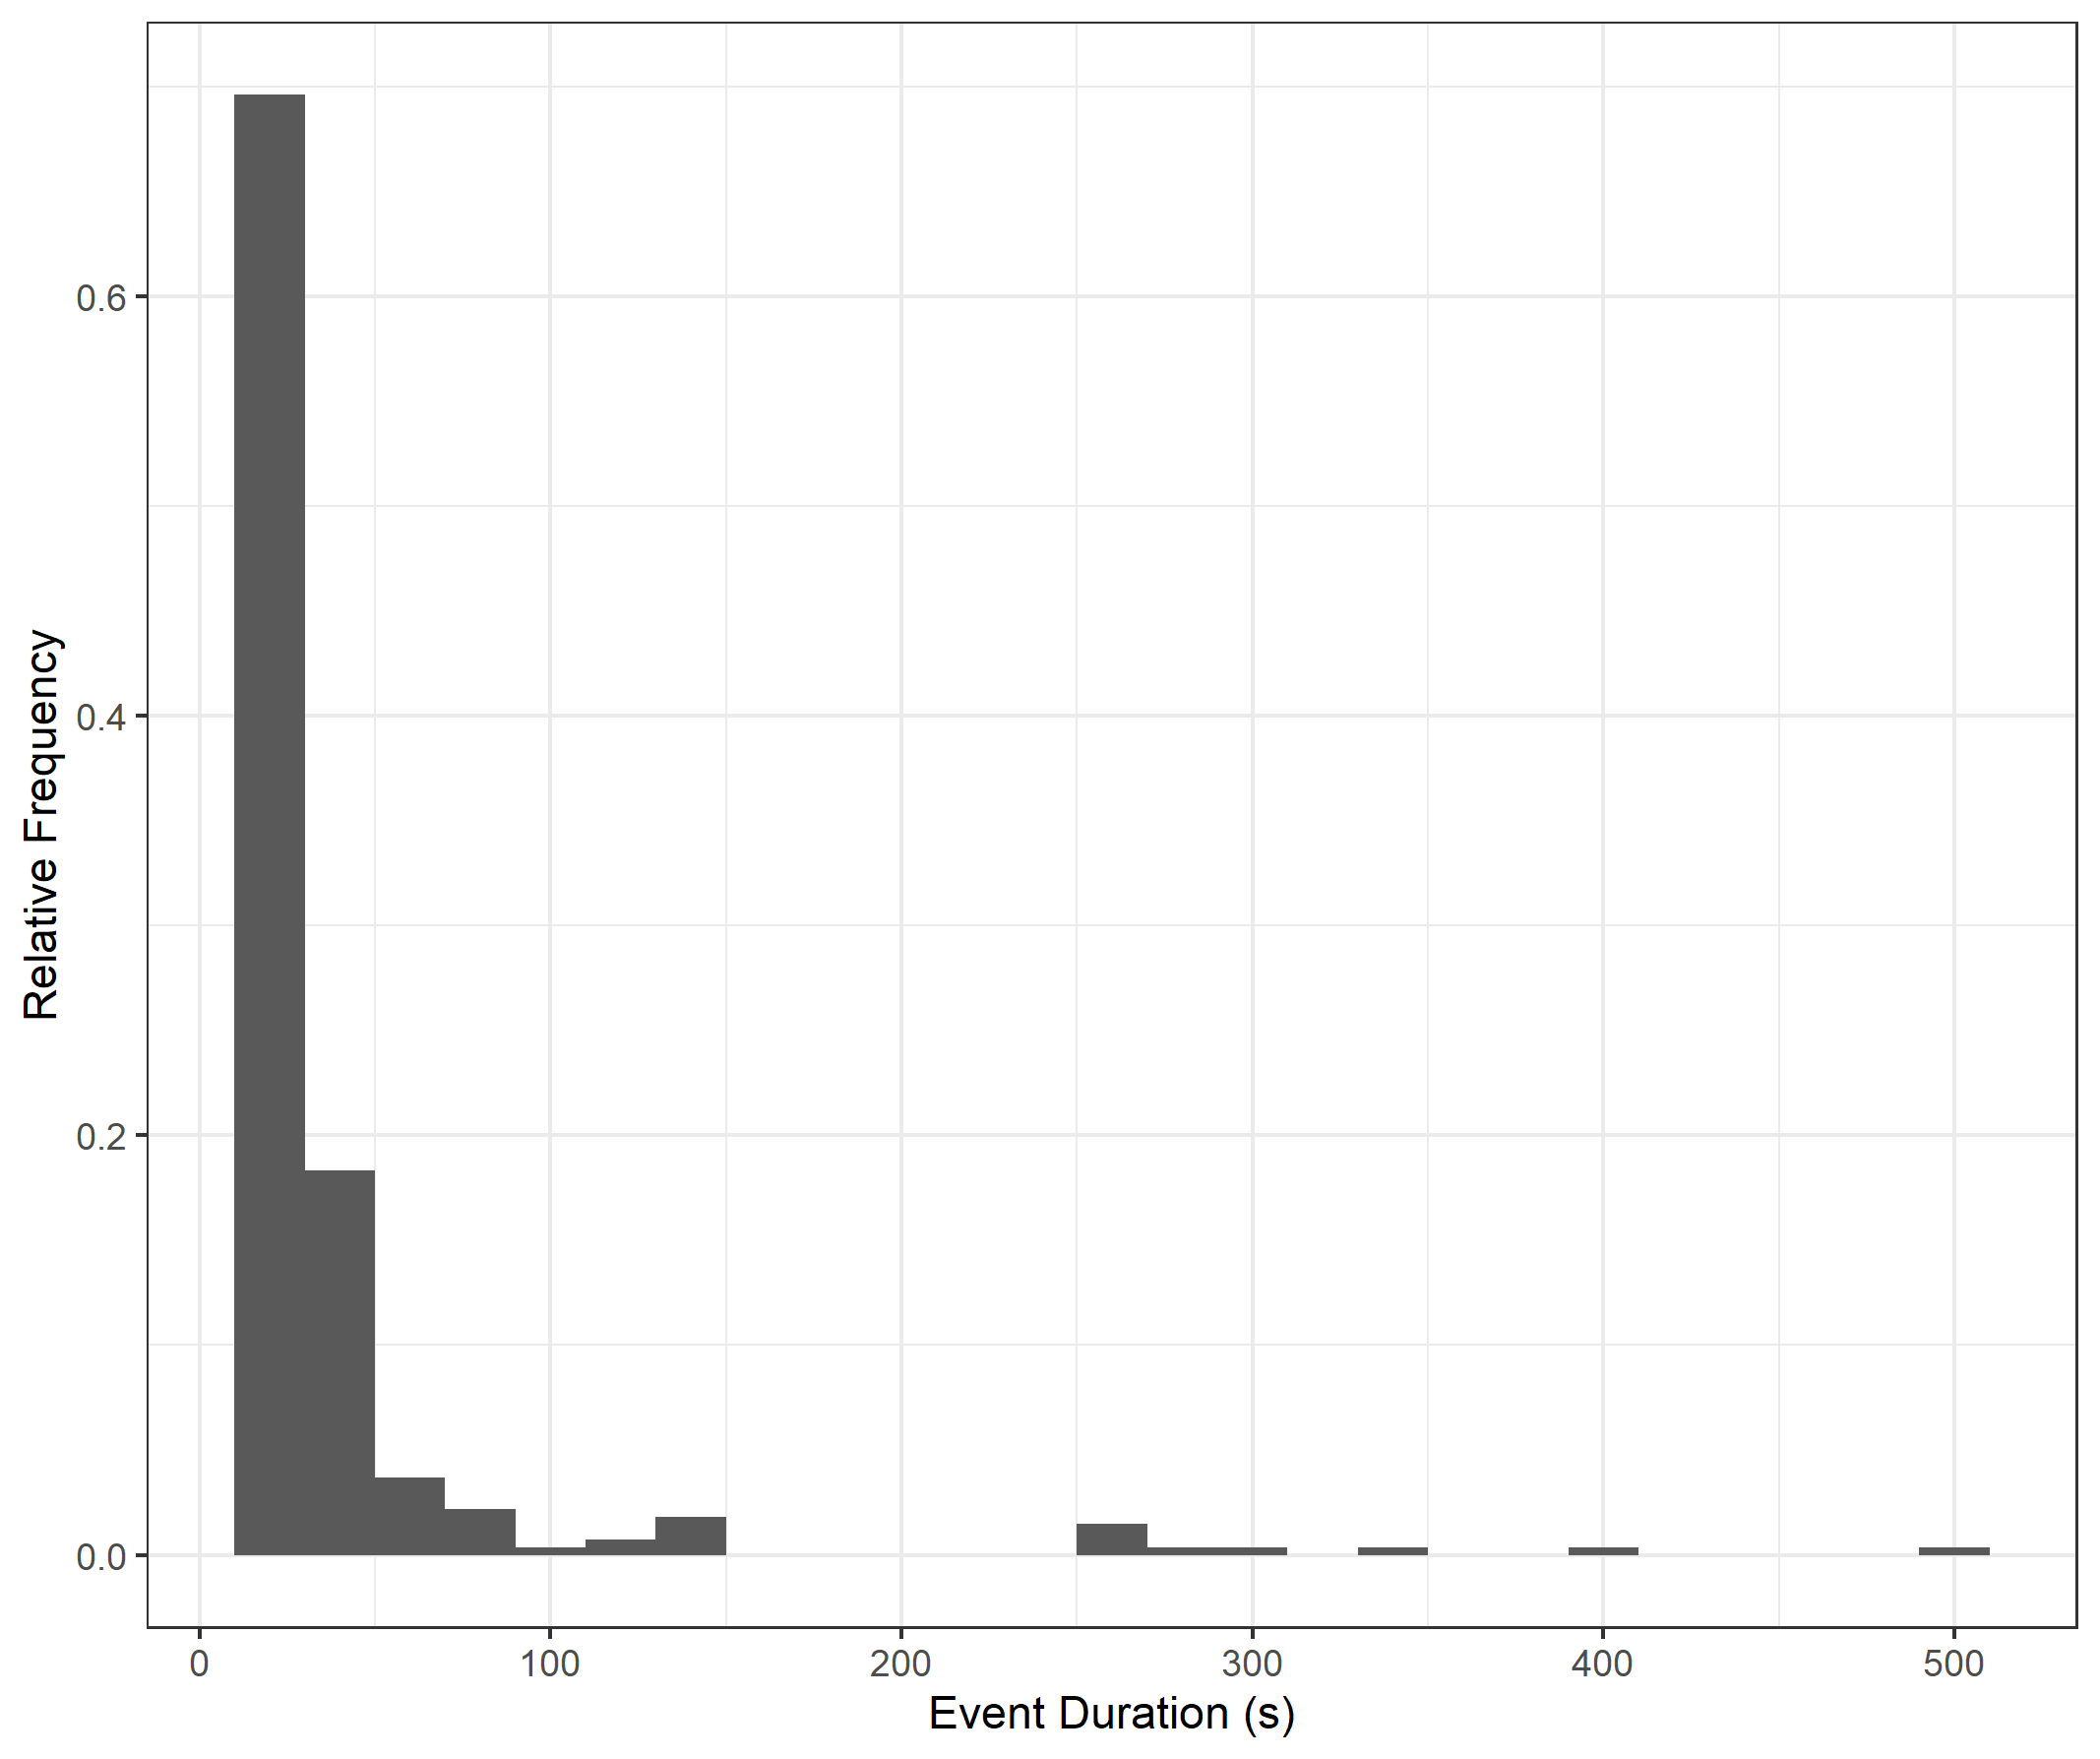
\includegraphics[width=0.6\textwidth]{images/integration/delta3.png}
\caption{Relative frequency histogram of the time it takes the kubernetes cluster to have the newly created consumers "ready".}
\label{fig:controller_result_kubernetes}
\end{figure}

After discarding the data points that didn't have the controller creating any
new consumer, there remain 273 data points, which show two clusters of data
points that are justified by two different scenarios when creating a new pod. 

The first, and most frequent (88\%), has the GKE cluster taking between $[10,
50]$ seconds to have a new consumer instance ready. This is usually the case when the
controller requests for the creation of new consumer instances and the
Kubernetes cluster has resources available to schedule the new consumer
instance. As such, the event's duration is related to the time it takes the
scheduled node(s) to download the image from the container registry, and to
start the containers.

The second group of data points, any time span greater than $50s$ (represents
12\% of the data points), occurs when the Kubernetes cluster does not have any
available resources. Here the actions the cluster undergoes are adding a new
node, and only then scheduling the consumer instance into the new available
node. Due to the autoscaling feature of the GKE cluster, this is done
automatically but it is also more inconsistent, having data points taking up to
$500s$, although very sporadically.

Although there isn't much control over the time it takes the Kubernetes cluster
to schedule and start the pods, one variable that can be controlled is the size
of the image which has to be downloaded by the nodes that were assigned the
newly created consumer instances.

\section{Communicating Change in State}

Each partition that the controller is monitoring can either be associated with a
start, stop, rebalance or a do nothing action. A start action refers to the case
where there is no consumer currently consuming data from the partition, and the
controller has assigned that partition to a consumer in its newly computed
consumer group state. The stop action occurs when the controller no longer wants
a consumer assigned to this partition therefore having no consumer fetching data
from this partition in the group's future state. 

Rebalancing happens when the controller is changing the partition from being
assigned from one consumer to another. Lastly, as the name suggest, do nothing
is when there are no actions to be communicated for a partition by the
controller to a consumer of the consumer group. Since there is no concurrent
read from the partition when the controller is analyzing a start or a stop
action, the controller can send this message as soon as it enters this event,
having to wait at most for 1 consumer cycle to receive the acknowledgement by
the consumer. 

When rebalancing, the controller has to first send out the stop command, wait
for a response, send out the start command, and wait for the response. Without
taking into account any processing and network delays, at worst, the controller
might have to wait for 2 consumer cycles to be able to rebalance a partition.

\begin{figure}[htb!]
\centering
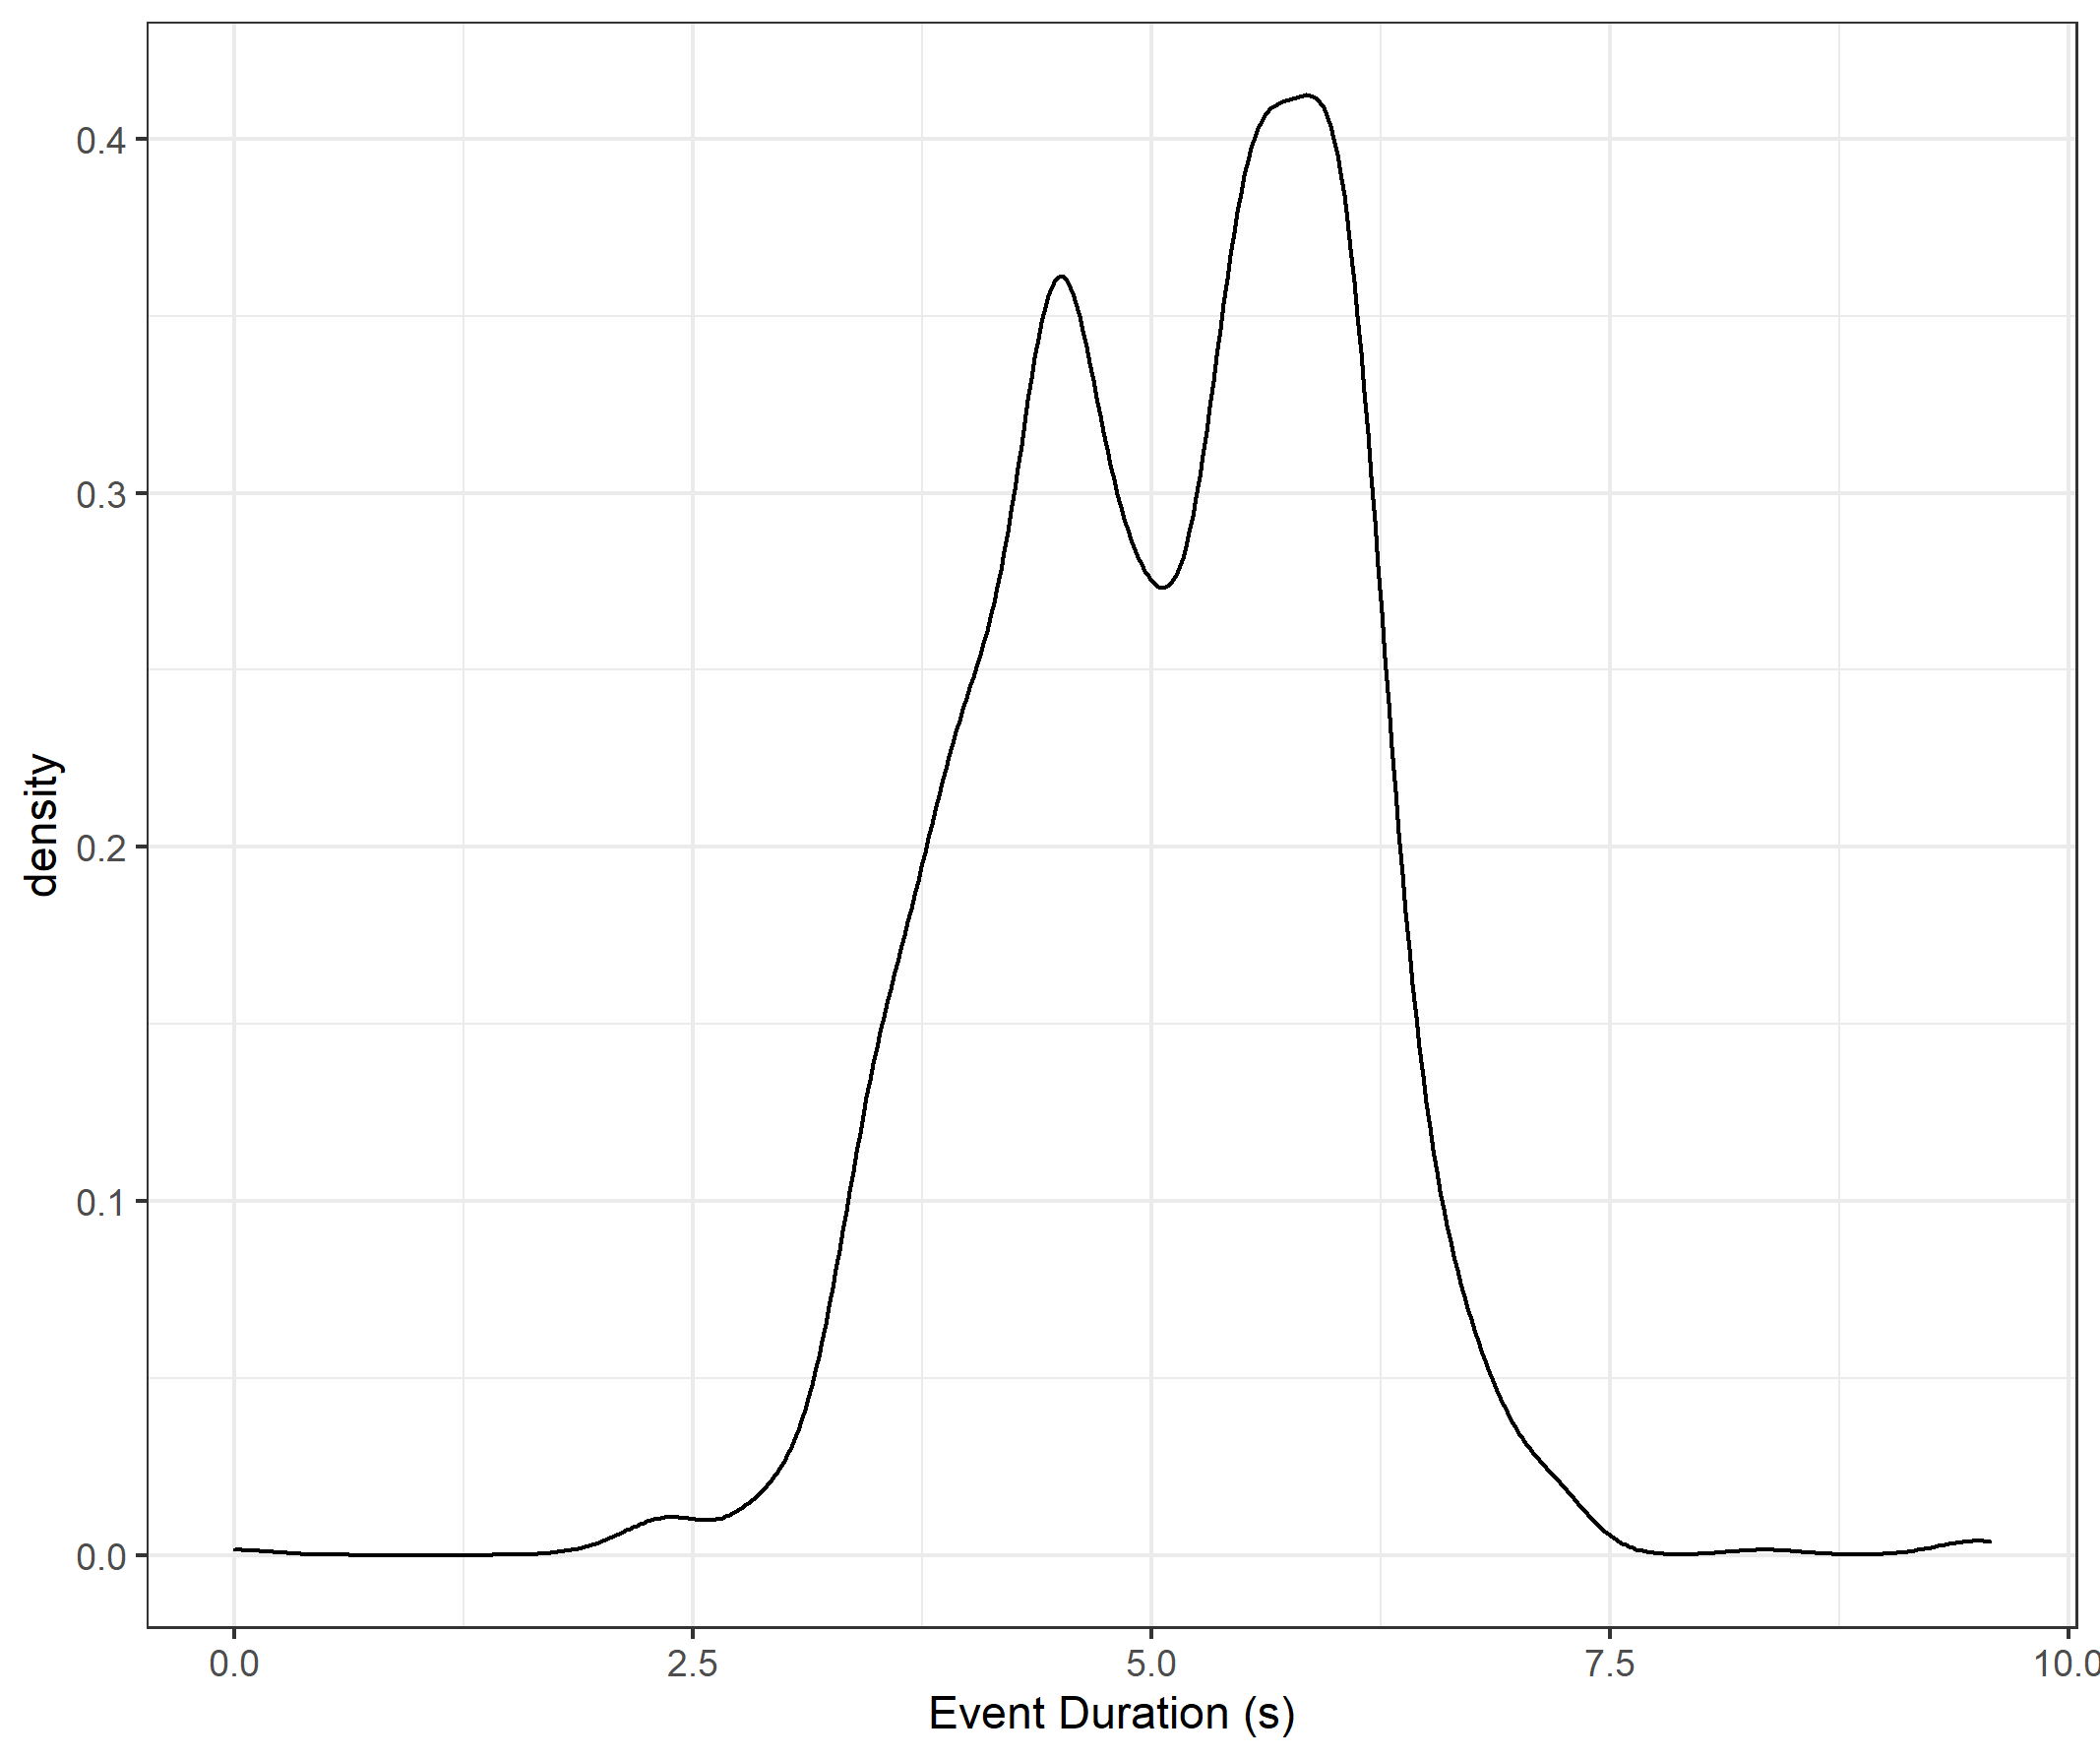
\includegraphics[width=0.6\textwidth]{images/integration/delta4.png}
\caption{
    Distribution of the time it takes the controller to communicate the change
    in state to its consumer group.
}
\label{fig:controller_result_change_state}
\end{figure}

A consumer's insert cycle goes through the different phases mentioned in section
\ref{component:consumer}, and only after performing it's tasks does it verify
the metadata queue to check if it has received any change in state command. For
this reason, between two metadata reads from the data-engineering-controller
topic, it takes the consumer 1 whole insert cycle. Having defined in section
\ref{c3subsub:consumer_maximum_capacity} that the consumer gathers at most
$5Mbytes$ per cycle, and provided the results from figure
\ref{fig:consumer_capacity}, which indicate the consumer has a data rate of
approximately $2Mbytes/s$, each consumer cycle can take approximately $2.5s$.
Since the controller has to wait for 2 consumer cycles, this would imply that
changing the group's state could take at least 5 seconds, as can be seen in figure
\ref{fig:controller_result_change_state}

It is also worth noting that the more consumers there are in the group, the
higher the probability that the consumer has to wait 1 whole cycle after sending
out the stop command, and another whole cycle after a start command, as the
communication is performed with more consumers.

Although this analysis was performed for a single partition, without any loss of
generality and due to the fact that the controller sends out the change state
commands in batch, the time it takes the controller to change a consumer group's
state remains at 2 consumer cycles.

To vary the duration of this event, the consumer's cycle has to be altered using
the \lstinline[language=Python]{BATCH_BYTES} and
\lstinline[language=Python]{WAIT_TIME_SECS} parameters, which in turn have an
effect on the time the consumer spends in a whole insert cycle.
